\documentclass{article}
\usepackage[utf8]{inputenc}
\usepackage{amsmath}
\usepackage{amsfonts}
\usepackage{amssymb}
\usepackage{graphicx}

\title{Equivalencia de las Condiciones de Integrabilidad de Riemann}
\author{Miguel Andrés Cazorla Zamora \\ Alexander Gutiérrez}
\date{}

\begin{document}
    \maketitle
	\section{Introducción}
	En el análisis matemático, la integrabilidad de Riemann es un concepto central en el estudio de funciones reales. Este documento presenta una demostración rigurosa de la equivalencia entre tres condiciones fundamentales para determinar la integrabilidad de Riemann de una función acotada definida en un intervalo cerrado. Estas condiciones son: la condición de Riemann, la condición de Darboux y la condición de Cauchy. La demostración de esta equivalencia proporciona un criterio robusto y versátil para establecer la integrabilidad de una función en el sentido de Riemann.
	\section{Interpretación Geométrica}
    A medida que la partición se vuelve más fina, es decir, $|P| \to 0$, la diferencia entre las sumas superior e inferior se hace arbitrariamente pequeña. Geométricamente, esto significa que las áreas superior e inferior convergen hacia un mismo valor, que es el valor de la integral.

\begin{center}
    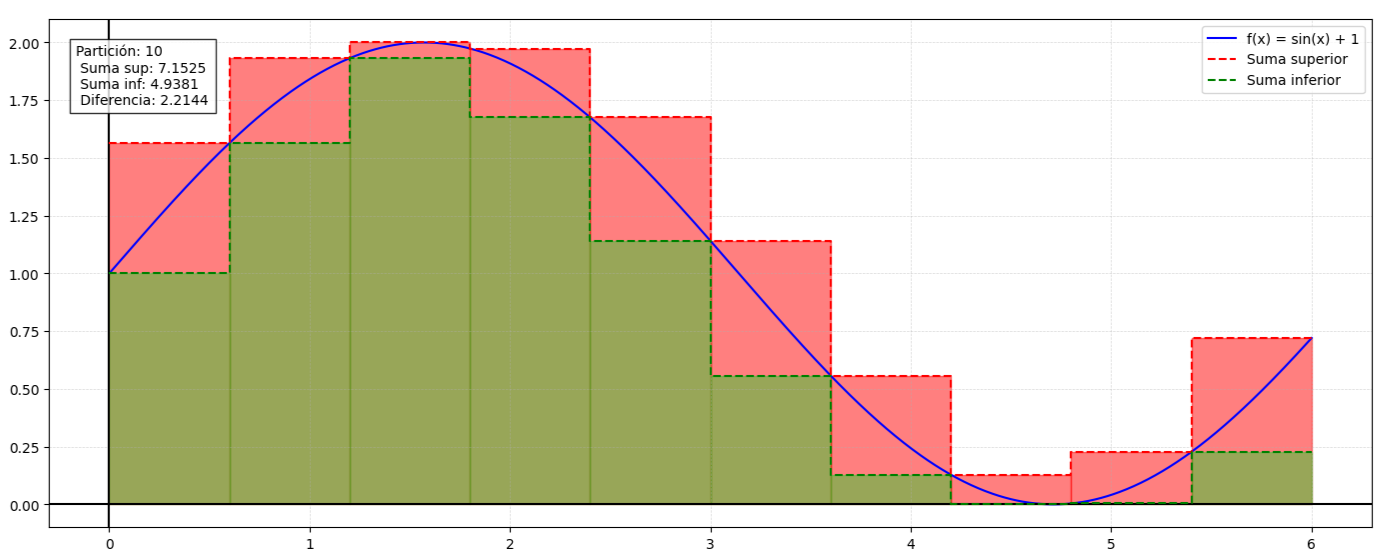
\includegraphics[width=1\textwidth]{Figure_1.png}
\end{center}
    
\begin{center}
    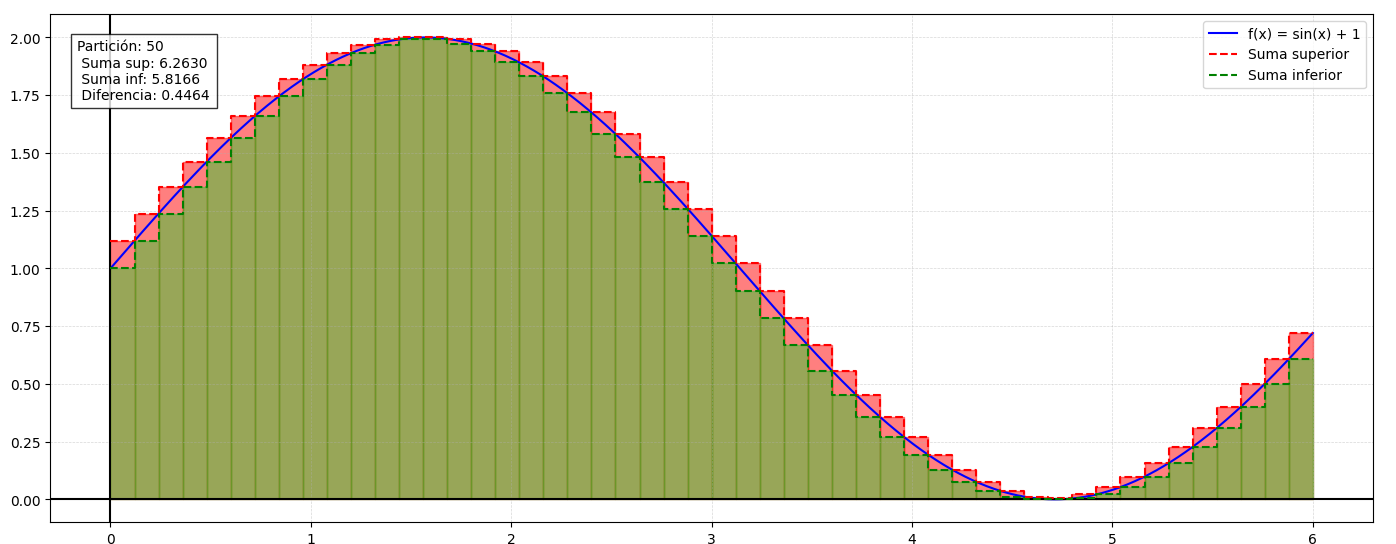
\includegraphics[width=1\textwidth]{Figure_2.png}
\end{center}

\begin{center}
    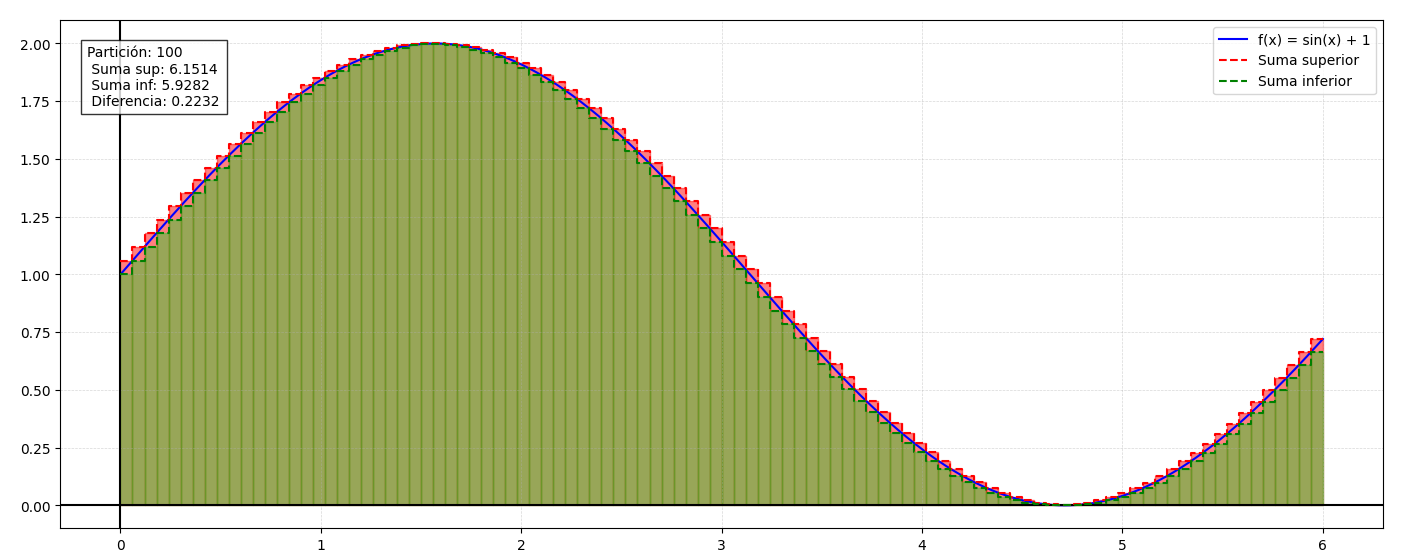
\includegraphics[width=1\textwidth]{Figure_3.png}
\end{center}

\section{Definiciones Preliminares}
	Sea $f: [a, b] \rightarrow \mathbb{R}$ una función acotada definida en un intervalo cerrado $[a, b]$.
	
	\begin{itemize}
		\item \textbf{Partición:} Una partición $P$ del intervalo $[a, b]$ es un conjunto ordenado de puntos $\{x_0, x_1, ..., x_n\}$ tal que $a = x_0 < x_1 < ... < x_n = b$.
		
		\item \textbf{Norma de una Partición:} La norma de la partición $P$, denotada por $\|P\|$, se define como $\|P\| = \max_{1 \leq i \leq n} (x_i - x_{i-1})$.
		
		\item \textbf{Suma Superior de Darboux:} La suma superior de Darboux de $f$ con respecto a la partición $P$ se define como $U(P, f) = \sum_{i=1}^{n} M_i (x_i - x_{i-1})$, donde $M_i = \sup\{f(x) : x \in [x_{i-1}, x_i]\}$.
		
		\item \textbf{Suma Inferior de Darboux:} La suma inferior de Darboux de $f$ con respecto a la partición $P$ se define como $L(P, f) = \sum_{i=1}^{n} m_i (x_i - x_{i-1})$, donde $m_i = \inf\{f(x) : x \in [x_{i-1}, x_i]\}$.
		
		\item \textbf{Integrabilidad de Riemann:} Una función $f$ se dice Riemann integrable en $[a, b]$ si $\exists\ I \in \mathbb{R}\ \forall\ \epsilon > 0$, $\exists$ una partición $P$ de $[a, b]$ tal que $|U(P, f) - L(P, f)| < \epsilon$. El número $I$ se llama la integral de Riemann de $f$ en $[a, b]$, denotada por $\int_{a}^{b} f(x) dx$.
	\end{itemize}
	
	\section{Condiciones de Integrabilidad de Riemann}
	\begin{enumerate}
		\item \textbf{Condición de Riemann:} $\forall\ \epsilon > 0$, $\exists$ una partición $P$ de $[a, b]$ tal que $U(P, f) - L(P, f) < \epsilon$.
		
		\item \textbf{Condición de Darboux:} $\lim_{\|P\| \to 0} U(P, f) = \lim_{\|P\| \to 0} L(P, f)$.
		
		\item \textbf{Condición de Cauchy:} $\forall\ \epsilon > 0$, $\exists$ una partición $P$ de $[a, b]$ tal que $\forall$ partición $P'$ que es un refinamiento de $P$ (es decir, $P' \supseteq P$), se cumple que $U(P', f) - L(P', f) < \epsilon$.
	\end{enumerate}
	
	\section{Demostración de la Equivalencia}
	Demostraremos la equivalencia de estas condiciones probando las siguientes implicaciones:
	$$ \text{Riemann} \Rightarrow \text{Darboux} \Rightarrow \text{Cauchy} \Rightarrow \text{Riemann} $$
	
	\subsection{Riemann $\Rightarrow$ Darboux}
	\textbf{Hipótesis:} $\forall\ \epsilon > 0$, $\exists$ una partición $P$ de $[a, b]$ tal que $U(P, f) - L(P, f) < \epsilon$.
	
	\textbf{Tesis:} $\lim_{\|P\| \to 0} U(P, f) = \lim_{\|P\| \to 0} L(P, f)$.
	
	\textbf{Demostración:} Dado $\epsilon > 0$, por hipótesis, existe una partición $P$ tal que $U(P, f) - L(P, f) < \epsilon$. Dado que $U(P, f)$ y $L(P, f)$ son, respectivamente, cotas superior e inferior de la integral de Riemann, se tiene que:
	
	$$ L(P, f) \leq \int_{a}^{b} f(x) dx \leq U(P, f) $$
	
	Al hacer $\|P\| \to 0$, las sumas superior e inferior convergen al mismo valor, lo cual demuestra la tesis.
	
	\subsection{Darboux $\Rightarrow$ Cauchy}

	\textbf{Hipótesis:} $\lim_{\|P\| \to 0} U(P, f) = \lim_{\|P\| \to 0} L(P, f)$.
	
	\textbf{Tesis:} $\forall\ \epsilon > 0$, $\exists$ una partición $P$ de $[a, b]$ tal que $\forall$ partición $P' \supseteq P$, se cumple que $U(P', f) - L(P', f) < \epsilon$.
	
	\textbf{Demostración:} Dado $\epsilon > 0$, por la condición de Darboux, existe $\delta > 0$ tal que para cualquier partición $P$ con $\|P\| < \delta$, se cumple que $U(P, f) - L(P, f) < \epsilon$.
	
	Si $P'$ es un refinamiento de $P$, entonces $\|P'\| \leq \|P\| < \delta$, por lo que la desigualdad sigue siendo válida. Esto demuestra que se cumple la condición de Cauchy.
	
	\subsection{Cauchy $\Rightarrow$ Riemann}

	\textbf{Hipótesis:} $\forall\ \epsilon > 0$, $\exists$ una partición $P$ de $[a, b]$ tal que $\forall$ partición $P' \supseteq P$, se cumple que $U(P', f) - L(P', f) < \epsilon$.
	
	\textbf{Tesis:} $\forall\ \epsilon > 0$, $\exists$ una partición $P$ de $[a, b]$ tal que $U(P, f) - L(P, f) < \epsilon$.
	
	\textbf{Demostración:} Dado $\epsilon > 0$, por la hipótesis (condición de Cauchy), existe una partición $P$ tal que para toda partición $P' \supseteq P$, se cumple que:
	
	$$ U(P', f) - L(P', f) < \epsilon $$
	
	En particular, tomando $P' = P$, se concluye que $U(P, f) - L(P, f) < \epsilon$, lo cual demuestra la tesis y, por lo tanto, que la función es integrable en el sentido de Riemann.
	
	\section{Conclusión}
	En este documento, hemos demostrado rigurosamente la equivalencia entre las condiciones de Riemann, Darboux y Cauchy para la integrabilidad de Riemann de una función acotada en un intervalo cerrado. Específicamente, hemos probado las siguientes implicaciones:
	
	$$ \text{Riemann} \Rightarrow \text{Darboux} \Rightarrow \text{Cauchy} \Rightarrow \text{Riemann} $$
	
	Por lo tanto, concluimos que estas tres condiciones son equivalentes:
	
	$$ \text{Riemann} \Leftrightarrow \text{Darboux} \Leftrightarrow \text{Cauchy} $$
	
	Este resultado establece que una función $f$ es Riemann integrable en $[a, b]$ si y solo si cumple cualquiera de estas condiciones, proporcionando un criterio robusto y versátil para determinar su integrabilidad. La equivalencia demostrada no solo enriquece nuestra comprensión teórica de la integrabilidad de Riemann, sino que también ofrece herramientas prácticas para la resolución de problemas y la extensión de conceptos en el análisis matemático.
\end{document}
